\section{Barycentric coordinates}
Barycentric coordinates, discovered by Möbius in 1827, consist of one of the most progessive area of research in computer graphics and mathematics thanks to the numerous applications in image and geometry processing.
% cite : http://lgg.epfl.ch/publications/2014/LBC/LBC.pdf
% ------
The position of any point in a triangle can be expressed using a linear combination with three scalars using barycentric coordinates:
$$ p = \lambda_1 p_1 + \lambda_2 p_2 + \lambda_3 p_3$$
where $p_1$, $p_2$ and $p_3$ are the vertices of a triangle and $\lambda_1$, $\lambda_2$ and $\lambda_3$ (the barycentric coordinates) are three scalars such that
respect the following barycentric coordinates properties.
% cite : https://www.scratchapixel.com/lessons/3d-basic-rendering/ray-tracing-rendering-a-triangle/barycentric-coordinates
% -------
\begin{itemize}
  \item partition of unity: $\sum_{i=1}^3 \lambda_{i}(p) = 1$
  \item reproduction: $\sum_{i=1}^3 \lambda_{i}(p)p_i = p$
  \item Lagrange-property: $\lambda_i(p_j) = \delta_{i, j}$
  \item linearity: $\lambda_i \in \prod_1$
  \item non-negativity: $\lambda_i(p)\geq 0$ for $p \in [p_1, p_2, p_3]$
\end{itemize}
%cite : https://www.icorsi.ch/pluginfile.php/406215/mod_resource/content/7/Graphics.2017.10.05.pdf
% -------
The point is inside the triangle if $0 \leq \lambda_1, \lambda_2, \lambda_3 \leq 1$. If a barycentric coordinates is less than zero or greater than one, the point is outside the triangle.
% cite : https://www.scratchapixel.com/lessons/3d-basic-rendering/ray-tracing-rendering-a-triangle/barycentric-coordinates
% -------
Barycentric coordinates allow to interpolate values from a set of control points over the interior of a domain, using weighted combinations of values associated with the control points (Fig. \ref{fig:barycentric-coord}).
% cite : http://lgg.epfl.ch/publications/2014/LBC/LBC.pdf
% ------
\begin{figure}
  \centering
  \scalebox{.7}{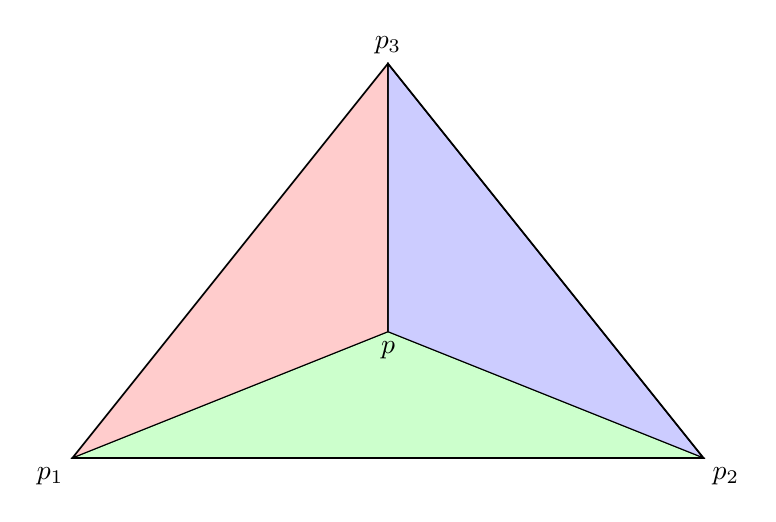
\begin{tikzpicture}
    \coordinate (L1) at (0,0);
    \coordinate (L2) at (8,0);
    \coordinate (L3) at (4,5);
    \coordinate (X) at (4,1.6);

    \draw[thick] (L1) -- coordinate[midway](md3) (L2)
                      -- coordinate[midway](md1) (L3)
                      -- coordinate[midway](md2) (L1) -- cycle;
    \filldraw[draw=black, fill=green!20] (L1) -- (X) -- (L2) -- cycle;
    \filldraw[draw=black, fill=red!20] (L1) -- (X) -- (L3) -- cycle;
    \filldraw[draw=black, fill=blue!20] (L3) -- (X) -- (L2) -- cycle;
    \draw (L1) node [below left] {$p_1$}
       -- (L2) node [below right] {$p_2$}
       -- (L3) node [above] {$p_3$}
       -- (X) node [below] {$p$};
    \end{tikzpicture}}
    \caption{Let $w_1$ be the red area, $w_2$ the green one and $w_3$ the blue one. Normalizing each of them by the area of the triangle, we will get three values ($\lambda_1, \lambda_2, \lambda_3$) that are the barycentric coordinates of $p$ with respect to the triangle [$p_1, p_2, p_3$].}
    \label{fig:barycentric-coord}
  \end{figure}

%%%%%%%%%%%%%%%%%%%%%%%%%%%%%%%%%%%%%%%%%%%%%%%%%%%%%%%%%%%%%%%%%

\section{Triangle meshes}
A collection of triangles without any particular mathematical structure are called \textit{triangle meshes} in many geometry processing algorithms. To derive a global parameterization for an entire triangle mesh we can define a 2D position for each vertex. Let be $\mathcal{M}$ a triangle mesh that consists of a geometric and topological component represented by a graph structure with a set of vertices $\mathcal{V} = \{ v_1, ..., v_V \}$ and a set of triangular faces connecting them $\mathcal{F} = \{ f_1, ... , f_F \}$ with $f_i \in \mathcal{V} \times \mathcal{V} \times \mathcal{V}$. The connectivity of a triangle mesh can be expressed in termes of the edges of the respective graph $\mathcal{E} = \{ e_1, ..., e_E \}$ where $e_i \in \mathcal{V} \times \mathcal{V}$.
% cite: Botsch 2010 Polygon Mesh Processing

%%%%%%%%%%%%%%%%%%%%%%%%%%%%%%%%%%%%%%%%%%%%%%%%%%%%%%%%%%%%%%%%%

\section{Lighting}
formula + draw and explanation of angle (like at 90 degree some light..e.tc.)
todo

%%%%%%%%%%%%%%%%%%%%%%%%%%%%%%%%%%%%%%%%%%%%%%%%%%%%%%%%%%%%%%%%%

\section{Linear Interpolation}
The standard linear interpolated visualisation is made passing three attributes (colors) for each vertex of a triangle. OpenGL will interpolate linearly the colors. That is possible thanks to the barycentric coordinates that will tell how much of each color is being mixed at any position.

%%%%%%%%%%%%%%%%%%%%%%%%%%%%%%%%%%%%%%%%%%%%%%%%%%%%%%%%%%%%%%%%%

\section{Flat Shading}
todo

%%%%%%%%%%%%%%%%%%%%%%%%%%%%%%%%%%%%%%%%%%%%%%%%%%%%%%%%%%%%%%%%%

\section{Gouraud Shading}
\textit{Gouraud Shading} can be calculated in the \textit{vertex shader}. The main idea is to compute a normal at the vertex and an intensity for each vertex.
todo (?)

%%%%%%%%%%%%%%%%%%%%%%%%%%%%%%%%%%%%%%%%%%%%%%%%%%%%%%%%%%%%%%%%%

\section{Curvature}
\subsection{Gaussian Curvature}
The \textit{Gaussian curvature} $K$ is defined as the product of the principal curvatures (square of the geometric mean):
$$K=k_1k_2$$
where $k_1$ and $k_2$ are the principal directions. A basic interpretation should be to imagine the \textit{Gaussian curvature} like a logical \texttt{AND} since it will check if there is a curvature along both directions.
The curvature of a surface is characterized by the principal curvatures, the \textit{Gaussian curvature} and the \textit{mean curvature} are simply averages of them.
%cite: A quick and dirty introduction to the curvature of surfaces (brickisland.net/cs177/?p=144)
%---------
\begin{figure}[h]
  \centering
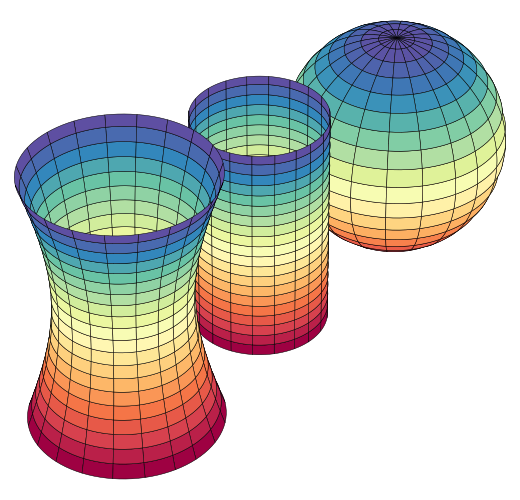
\includegraphics[scale=0.5]{images/gaussian_curvature_examples.png}
\caption{Negative curvature, zero curvature and positive curvature.}\label{fig:curvature-gaussian}
\end{figure}
% \begin{figure}[h]
%   \minipage[b]{.5\linewidth}
%   \centering
%   \scalebox{0.7}{\begin{tikzpicture}
%   \begin{axis}[view={60}{30}]
%       \addplot3[surf,shader=flat,
%           samples=20,
%           domain=1:0,y domain=0:2*pi,
%           z buffer=sort]
%           ({sqrt(1-x^2) * cos(deg(y))},
%        {sqrt( 1-x^2 ) * sin(deg(y))},
%        x);
%   \end{axis}
%   \end{tikzpicture}}
%   \caption{Positive GC}\label{fig:positive-gaussian}
%   \endminipage
%   \minipage[b]{.5\linewidth}
%   \centering
%   \begin{tikzpicture}[scale=0.7]
%     \begin{axis}[view={60}{30}]
%     \addplot3[patch,patch refines=3,
%     shader=faceted interp,
%     patch type=biquadratic]
%     table[z expr=x^2-y^2]
%     {
%         x  y
%         -2 -2
%         2  -2
%         2  2
%         -2 2
%         0  -2
%         2  0
%         0  2
%         -2 0
%         0  0
%     };
%   \end{axis}
%   \end{tikzpicture}
%   \caption{Negative GC}\label{fig:negative-gaussian}
%   \endminipage
% \end{figure}
Surfaces that have a zero gaussian curvature are called \textit{developable surfaces} because they can be flattened out into the plane without any stretching. \textit{Gaussian curvature} should be zero inside each mesh triangle and the same along edges since it can be flattened symmetrically into the plane by simply rotating one triangle about the common edge into the plane defined by the other. Consequently the \textit{Gaussian curvature} is concentrated at the vertices of a triangle and defined as the \textit{angle defect}
$$K(V) = 2 \pi - \sum_{i=1}^n \theta_i$$
where $\theta_i$ are the angles of the triangle $T_i$ adjacent to the vertex $V$ at $V$. This should be seen as the integral of the Gaussian curvature over a certain region $S(V)$ around $V$, where these $S(V)$ form a partition of the surface of the entire mesh.
$$ K(V) = \int_{S(V)} KdA  $$
\textit{Negative curvature} can be recognized by the fact that external directions curve in opposite directions, \textit{zero curvature} has one external direction that has zero curvature, \textit{positive curvature} has external directions that curve in the same direction (Fig. \ref{fig:curvature-gaussian}).
The \textit{Theorema Egregium}, discovered by C.F. Gauss in 1827, states that the \textit{Gaussian curvature} is an intrinsic property of the surface that does not depend on the space, despite by the fact that is define as the product of the principal curvatures (whose value depends on how the surface is immersed in the space). Technically, the \textit{Gaussian curvature} is invariant under isometries.
We can then notice that triangle angles add up to less than $180 \degree$ in negative curature, exactly $180 \degree$ in zero curature, and more than $180 \degree$ in positive curature.

%cite: Geometry Processing Kai Hormann (paper)


%%%%%%%%%%%%%%%%%%%%%%%%%%%%%%%%%%%%%%%%%%%%%%%%%%%%%%%%%%%%%%%%%

\subsection{Mean Curvature}
TODO


